% Characteristics of Individual Bees


Degree of a bee, the number of other bees this bee interacts with.
Strength


Degree, Strength and Local Clustering Coefficient and \\
Betweenness and Closeness Centrality\\
\\
bimodal degree distribution\\
type of network: no scale free\\
todo plot in relation to age of bees\\
todo plot in relation to detection frequency\\

\begin{figure}[!htb]
	\centering
	\begin{subfigure}[b]{1.0\textwidth}
	\centering
	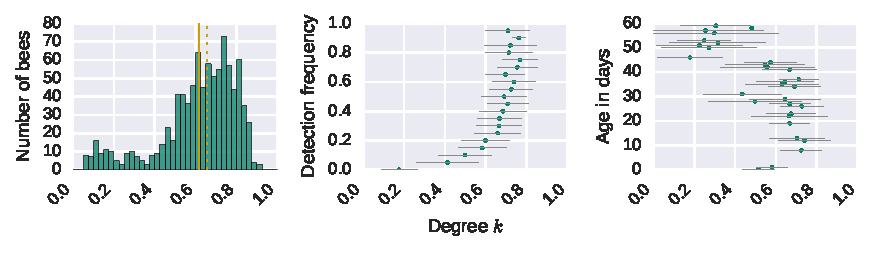
\includegraphics[width=1.0\textwidth]{Figures/n3-stat-degreeAgeDetF.pdf}
	\caption[Degree]{\textbf{Degree}}
	\label{fig:n3-degree}
	\end{subfigure}
	\begin{subfigure}[b]{1.0\textwidth}
	\centering
	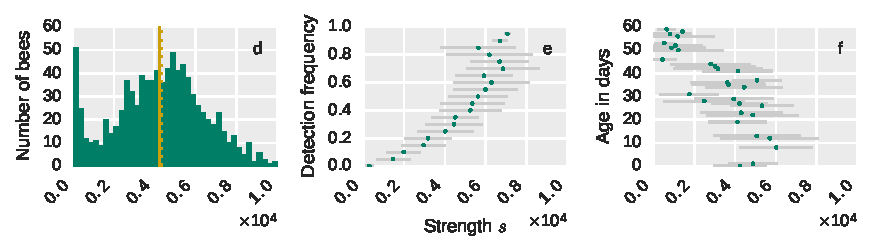
\includegraphics[width=1.0\textwidth]{Figures/n3-stat-strengthAgeDetF.pdf}
	\caption[Strength]{\textbf{Strength}}
	\label{fig:n3-strength}
	\end{subfigure}
	\begin{subfigure}[b]{1.0\textwidth}
	\centering
	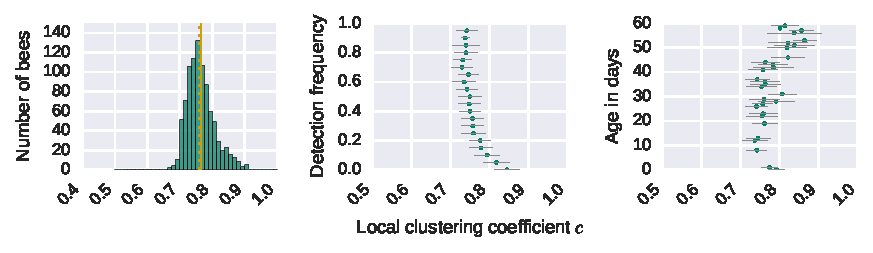
\includegraphics[width=1.0\textwidth]{Figures/n3-stat-lccAgeDetF.pdf}
	\caption[Local clustering coefficient]{\textbf{Local clustering coefficient}}
	\label{fig:n3-lcc}
	\end{subfigure}
	\caption[Degree, strength and local clustering coefficient (LCC)]{\textbf{Degree, strength and local clustering coefficient (LCC) in relation to age and detection frequency} xxx}
	\label{fig:n3-degreeStrLCC}
\end{figure}


[TODO]\\
in relation to age and detection frequency\\
closeness\\
betweenness\\

\begin{figure}[!htb]
	\centering
	\begin{subfigure}[b]{1.0\textwidth}
	\centering
	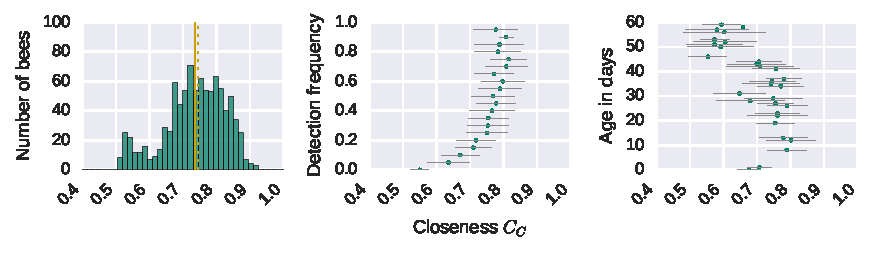
\includegraphics[width=1.0\textwidth]{Figures/n3-stat-closenessAgeDetF.pdf}
	\caption[Closeness Centrality]{\textbf{Closeness Centrality}}
	\label{fig:n3-closeness}
	\end{subfigure}
	\begin{subfigure}[b]{1.0\textwidth}
	\centering
	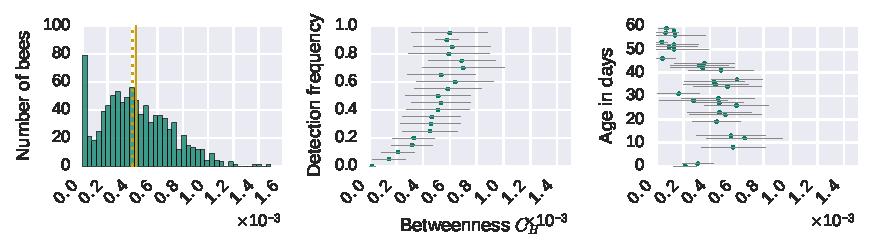
\includegraphics[width=1.0\textwidth]{Figures/n3-stat-betweenAgeDetF.pdf}
	\caption[Betweeness Centrality]{\textbf{Betweeness Centrality}}
	\label{fig:n3-between}
	\end{subfigure}
	\caption[Centrality]{\textbf{Centrality in relation to age and detection frequency} xxx}
	\label{fig:n3-centrality}
\end{figure}
